\documentclass{article}
\usepackage{amsmath}
\usepackage{epsfig}
\usepackage{cite}
\usepackage{graphicx}

\title{PacBio Assembly}
\author{XXX}

\begin{document}
\maketitle
\section{Introduction}

Most shotgun sequencing methods use huge amount of short fragments to assemble
the whole DNA sequence. However, new sequencing instruments from Pacific
Biosciences (PacBio) can sequence much longer fragments of DNA than any other
sequencing technology (2000bp compared to 100--500bp), but at a much higher
error rate (typically 15\% error). The long read length makes the instruments
very attractive for de novo assembly of complex genomes, but the high error rate
prevents traditional approaches from being used. Nevertheless, with high
coverage, it is still possible to eliminate the read errors and assembling the
whole genome from them.

Our team aims at assembling the genome of E-coli from PacBio's long sequence
reads with high error rate. Researcher in PacBio eliminated the errors by
aligning relatively short but accurate Circular Consensus Sequencing (CCS) reads
against those long reads. However, we proposed to assemble the genome using only
long reads, which is challenging but possible thanks to large coverage of the
reads.

The key issue of our problem is to efficiently and accurately detect
overlaps. Our approach employs the seed-and-extend paradigm, in which
spaced seed is used to sufficiently locate possibly overlapped
sequences. Sequence aligner is then applied to those candidates to work
out possible alignment. Once aligned, more precise sequence can be
obtained by consensus.

\section{Algorithm}

\subsection{Seed-and-extend}

Our algorithm iteratively aligns long reads to a reference, which represents all
sequences already aligned. During each alignment, the aligned reads will vote to
correct errors in the reference and expand it if they are at boundaries of the
reference. Eventually, the reference will be the genome or contigs we are
looking for. It is important to maintain the reference as accurate as possible,
        so that minimum structural errors will be introduced in the grow
        process. To guarantee this, the reference should start as an accurate
        sequence. There are several methods to get an initial high quality
        reference. One is to select those long reads with high average Phred
        quality scores, which are easily accessible in the FASTQ sequence files
        downloaded from DevNet of PacBio. Another method is to use a CCS
        corrected read, which is inherently of high accuracy. According to the
        data provided by PacBio, the mean accuracy of CCS read is 97.8.

During the extend process, it is most important that the extension comes
from a really overlapped sequence. Otherwise, there will be structural
errors in the reference, which will cause a wrong assembly or early
failure of iteration.

\subsection{Overlap detection}

Spaced seeds are used to find overlapped sequence that can be aligned to
the reference. To achieve this, we build a seedmap for the reference and
detect overlaps by looking up seeds from a candidate read into it. The
seedmap is a hashmap for all possible seeds of the reference, so look-up
into it is fast. Given a reference of length $n$ and a spaced seed with
length $k$ and weight $w$ (weight here is the number of 1s in the spaced
seed pattern, e.g., the weight of the 16-base-long seed pattern
\verb!111*11*1*1*1*111! is 11), there will be $n-k+1$ seeds, when the
seed pattern is applied to the reference at different places. For each
candidate read, there is no need to lookup all of its seeds because we
can safely rule it out if it fails a certain number of trials. The trial
of alignment always starts at one end of the sequence. So it is enough
to only look at seeds at both ends.

If there is a match of seed, there will be an attempt to align the sequence
against the reference. The alignment basically calculates the shortest edit
distance, which is a dynamic programming process with square order of
complexity. However, because we are only interested in those sequences with high
similarity to the reference. It is not neccessary to go through all elements in
the DP matrix.  Only the diagonal region of the matrix will be used and updated.
The average of error rate is 15\%, so the mutual difference will be around 30\%.
The time and space of the alignment will be $0.3n^2$. Because most sequences are
about 3000-base-long, the complexity of a typical successful alignment is around
900000. This is affordable on a modern computer.

It is desirable that the overlaps happen at the boundaries of the reference.
Because the reference can grow and the iteration will converge quickly. However,
        we should be careful since the length of overlapped region can be small.
        But overlap of a short region can happen frequently by accident
        considering the large scale of data. To avoid this situation, the
        alignment must be significant long to justify an overlap.

\subsection{Tradeoffs}

In our algorithm, several tradeoffs have been made to balance accuracy and
speed. Firstly, in the dynamic programming process, it is reasonable to quit and
report failure if the intermidate optimal distance becomes significantly large.
This early failure strategy will miss some overlaps with low match in the prefix
but high match as a whole, however, it will considerably accelerate the
alignment.

To converge quickly, it is absolutely favorable to detect all possible overlaps
during each iteration. However, this is quite difficult considering the high
error rate. Otherwise, the program greatly slows down when the reference becomes
long. If all seeds in the long reference are placed into the seedmap, the
probability of accident seed-matches will increase dramastically. Actually, our
algorithm aims at correcting errors and assembling sequences at the same time.
However, preference over assembling sequences is desirable at the early stage.
As long as we can grow the reference and obtain a rough overview structure, we
can correct the errors thereafter. To the opposite, if the reference cannot grow
smoothly, the iteration will fail at an early stage. We note that only overlaps
at boundaries are helpful for reference grow, we will only build seedmap for
both ends of the reference in the seedmap before the length of reference
approach the length of the genome. Therefore, the number of seed-matches will be
limited and the iteration period get shortened.

\section{Implementation}

We have implemented the algorithm using C++. It is public available at
https://github.com/brianchenming/PacBioAssembly. The long reads are ``E.
coli C227--11 Filtered Reads FASTQ'' from \\ 
http://www.pacbiodevnet.com/Share/Datasets/E-coli-Outbreak. 

The sequence files are 3G after decompression and DNA sequences contribute half
of the size, whereas the other half is quality string in the FASTQ format.  But,
   1.5G is still quite large and cannot fit into our laptop's memory.  However,
   we do not want to do too much disk IO becomes IO operations can significantly
   slow down the whole program. So we converted the DNA sequences into a binary
   file and decrease the memory assumption into a quarter of the size. The
   binary format is not only memory efficient, it also facilitates the
   calculation of spaced seeds. By carefully choosing the seed pattern to be of
   length 16, a seed can fit into one 32-bit (2 bits for one base) machine word,
   so a seed match is just a comparison of two unsigned integers. Using binary
   format, we can easy obtain seeds using bitwise operations on the sequence and
   the seed pattern. A class is created to provide interfaces of manipulating
   the binary format.

\subsection{Seedmap}

The seedmap is implemented as a hash\_map from the C++ standard template
library. Ideally, every time the reference gets updated by incorporating a new
read, its seedmap should be refreshed as well. But it is very time-consuming,
  especially when it becomes long in the late phases of the iteration. So, we
  made a tradeoff and only add elements into the seedmap in one iteration.
  First, let us consider the case of substitution. A `C' base at the $j$-th
  position of the reference may have been voted to become `G'. In our
  implementation, this change of consensus will not be reflected in the seedmap
  until next iteration.  This delay of update is not a big problem because
  missed overlaps can be detected in later iterations. Second, as to deletion,
  we can just ignore it because a deletion of a base it is just an absence of
  one vote at that position. We can delete the base if it gets significant less
  votes at the end of iteration. The third case, insertion, is the most
  difficult. For insertion at the two ends of the reference, it is easy because
  we can add new seed without invalidating the seedmap. It is difficult to
  handle insertion in the middle while keeps elements in the seedmap intact. In
  our implementation, we solved this by only allowing one insertion after each
  place. Alignments with overlaps may insert many bases after one position,
  however, no matter how many bases are inserted by whatever-number-of-overlaps,
  only one box is used for all of them.  For example, one read wants to insert
  `ACCG' after the $j$-th position of the reference, and another read wants to
  insert `GGT' at the same position, then the box reserved for insertion at that
  position will have votes `A:1, C:2, G:3, T:1'. If 3 is significant, there will
  be one additional `G' only after the current round terminates. The code for
  the overlaps detection is finished and partially tested, while the code for
  updating seedmap after alignment is drawing to an end.

\subsection{Program structure}

Besides seedmap, there are seven core classes as presented in Figure 1.
\emph{dna\_seq} is an abstration of DNA sequence and \emph{seq\_accessor}
capsulates methods to visit \emph{dna\_seq}.  \emph{seq\_aligner} is the class
responsible for aligning two sequences.  \emph{ref\_seq} represents the
reference it is also the place where \emph{vote\_box} resides. \emph{vote\_box}
is composed of two \emph{base\_vote}, one being selection and other being
suppliment.

\begin{figure}[t]
    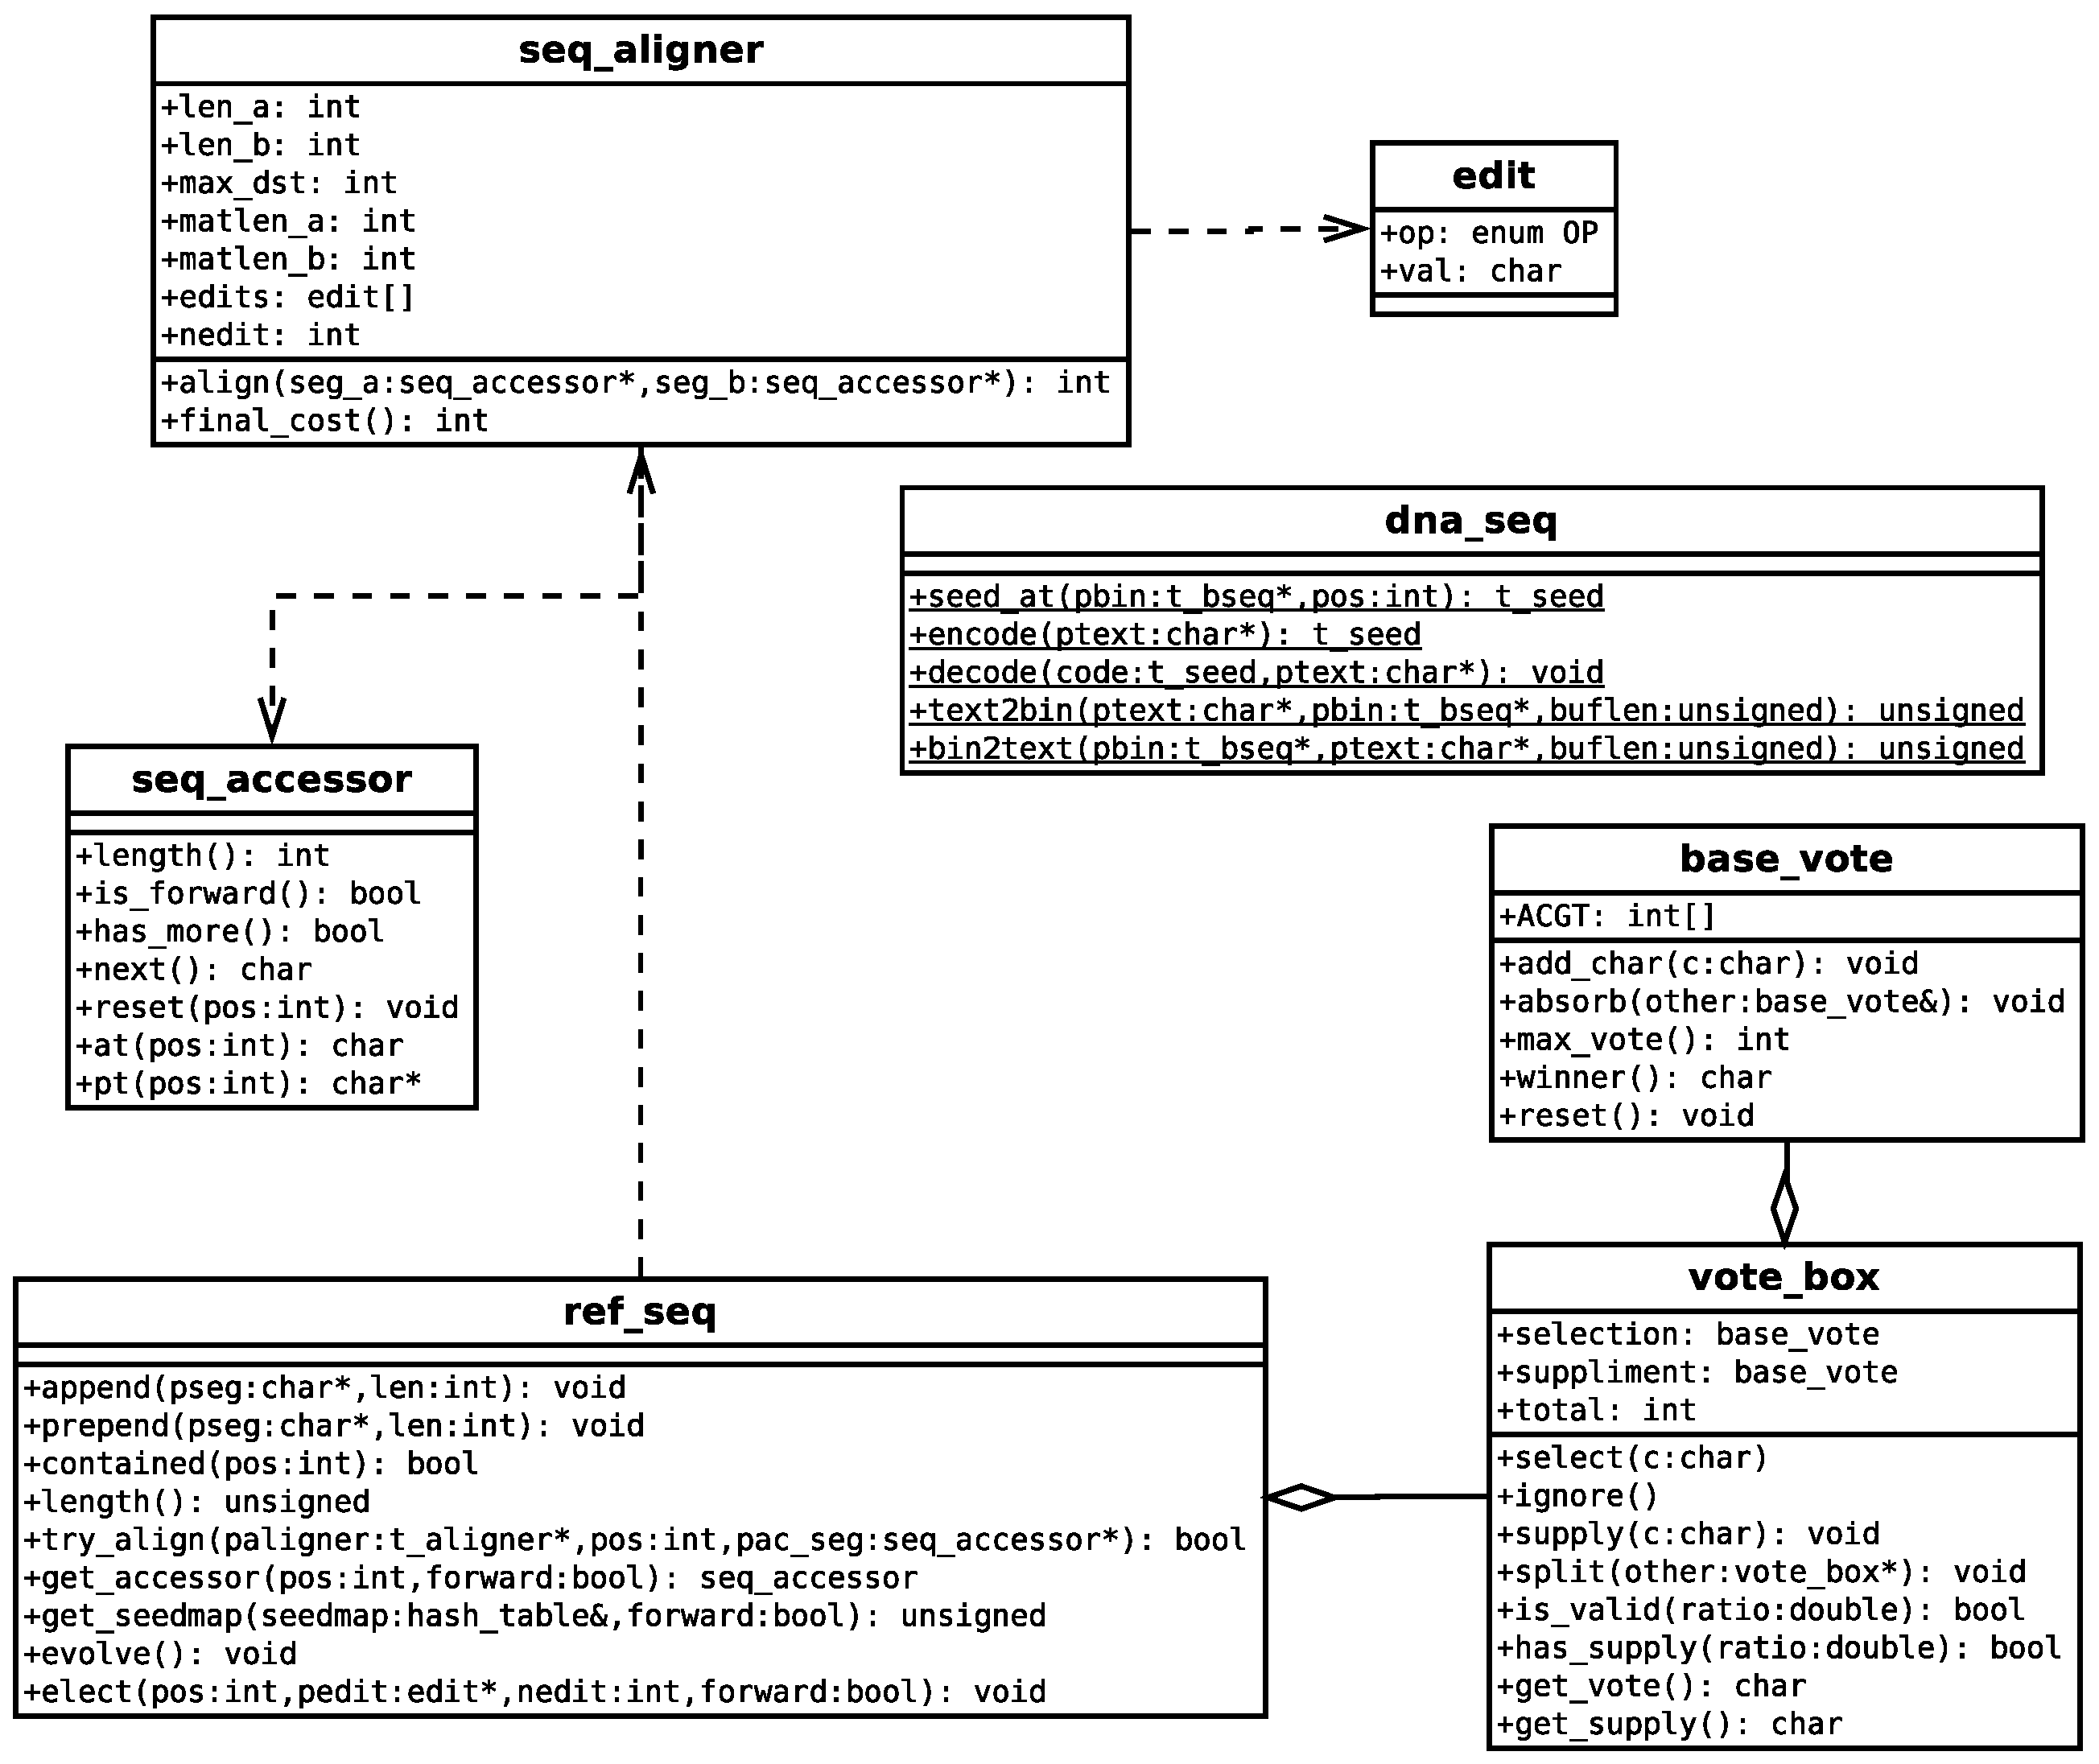
\includegraphics[width=12.5cm, keepaspectratio=true]{class.eps}
    \caption{\label{fig:compare}Class UML}
\end{figure}

\subsection{Testing}

Using GoogleTest, we have created comprehensive unit test cases for
these classes, especially \emph{seq\_aligner} and \emph{ref\_seq}. The
binary format has being tested on real data. We successfully converted
100M sequence into binary file and get the exact sequences back in text
format. The aligner has been tested on artificial data, long reads and
CCS reads. For the alignment, a \emph{visual\_align} program has also
been implemented to visualize alignment for manual examination.

\section{Experiment}

Experiments have been conducted to evaluate our program. Different data
sets and different parameters have been used in our experiments.

\subsection{Overlap detection}

Overlap detection is the most important part of our program. In the iteration,
        there is summary information for every detected overlap including the
        edit distance and the length of match in both reference and sequence. We
        can check this output and make sure the alignment are working properly.
        A real example of the information is shown in the following table.
        Moreover, an option has been provided in our program to dump all
        detected overlapped segments during the whole process. Therefore, we can
        use \emph{visual\_align} to manually examine the overlaps. In our
        examination, all overlapped pairs can be well aligned with each other.
        Some overlaps detected by our program from real data are attached.

\begin{center}
\begin{tabular}{lll}
Sequence ID Distance & Match In Ref & Match In Segments\\
\hline
found 161780 at cost 83: & ref\_ml=370, & seg\_ml=378\\
found 191077 at cost 50: & ref\_ml=232, & seg\_ml=239\\
found 28765 at cost 382: & ref\_ml=1442, & seg\_ml=1442\\
found 136441 at cost 347: & ref\_ml=1466, & seg\_ml=1607\\
found 206229 at cost 578: & ref\_ml=2231, & seg\_ml=2369\\
found 237917 at cost 1658: & ref\_ml=6119, & seg\_ml=6047\\
found 11519 at cost 69: & ref\_ml=264, & seg\_ml=264\\
found 88452 at cost 173: & ref\_ml=618, & seg\_ml=618\\
found 123619 at cost 1215: & ref\_ml=4380, & seg\_ml=4380\\
\end{tabular}
\end{center}

The precision of overlaps can be controlled by parameters to our aligner and can
be verified by above-mentioned techniques. However, the recall of overlaps is
more difficult to achieve but meanwhile more important. It determines the
success of our algorithm to a great degree. There are experiments on both CCS
reads and error reads for overlap detection. For CCS reads, the overlap
detection works very well. In the first 10 rounds of iteration of one
experiment, the average number of detected overlaps is 24.8. Near 25 overlaps in
each iteration is great because it provide abundant chances to grow the
reference and to correct errors. For error reads, the number of overlaps is much
less. In the first 10 rounds of iteration of one experiment, the average numbers
of overlaps are respectively 3.3 and 6 when the initial reference is from error
reads and CCS reads. What is worse, the number of overlaps decrease for error
reads while keep stable for CCS reads.

\begin{figure}[t]
    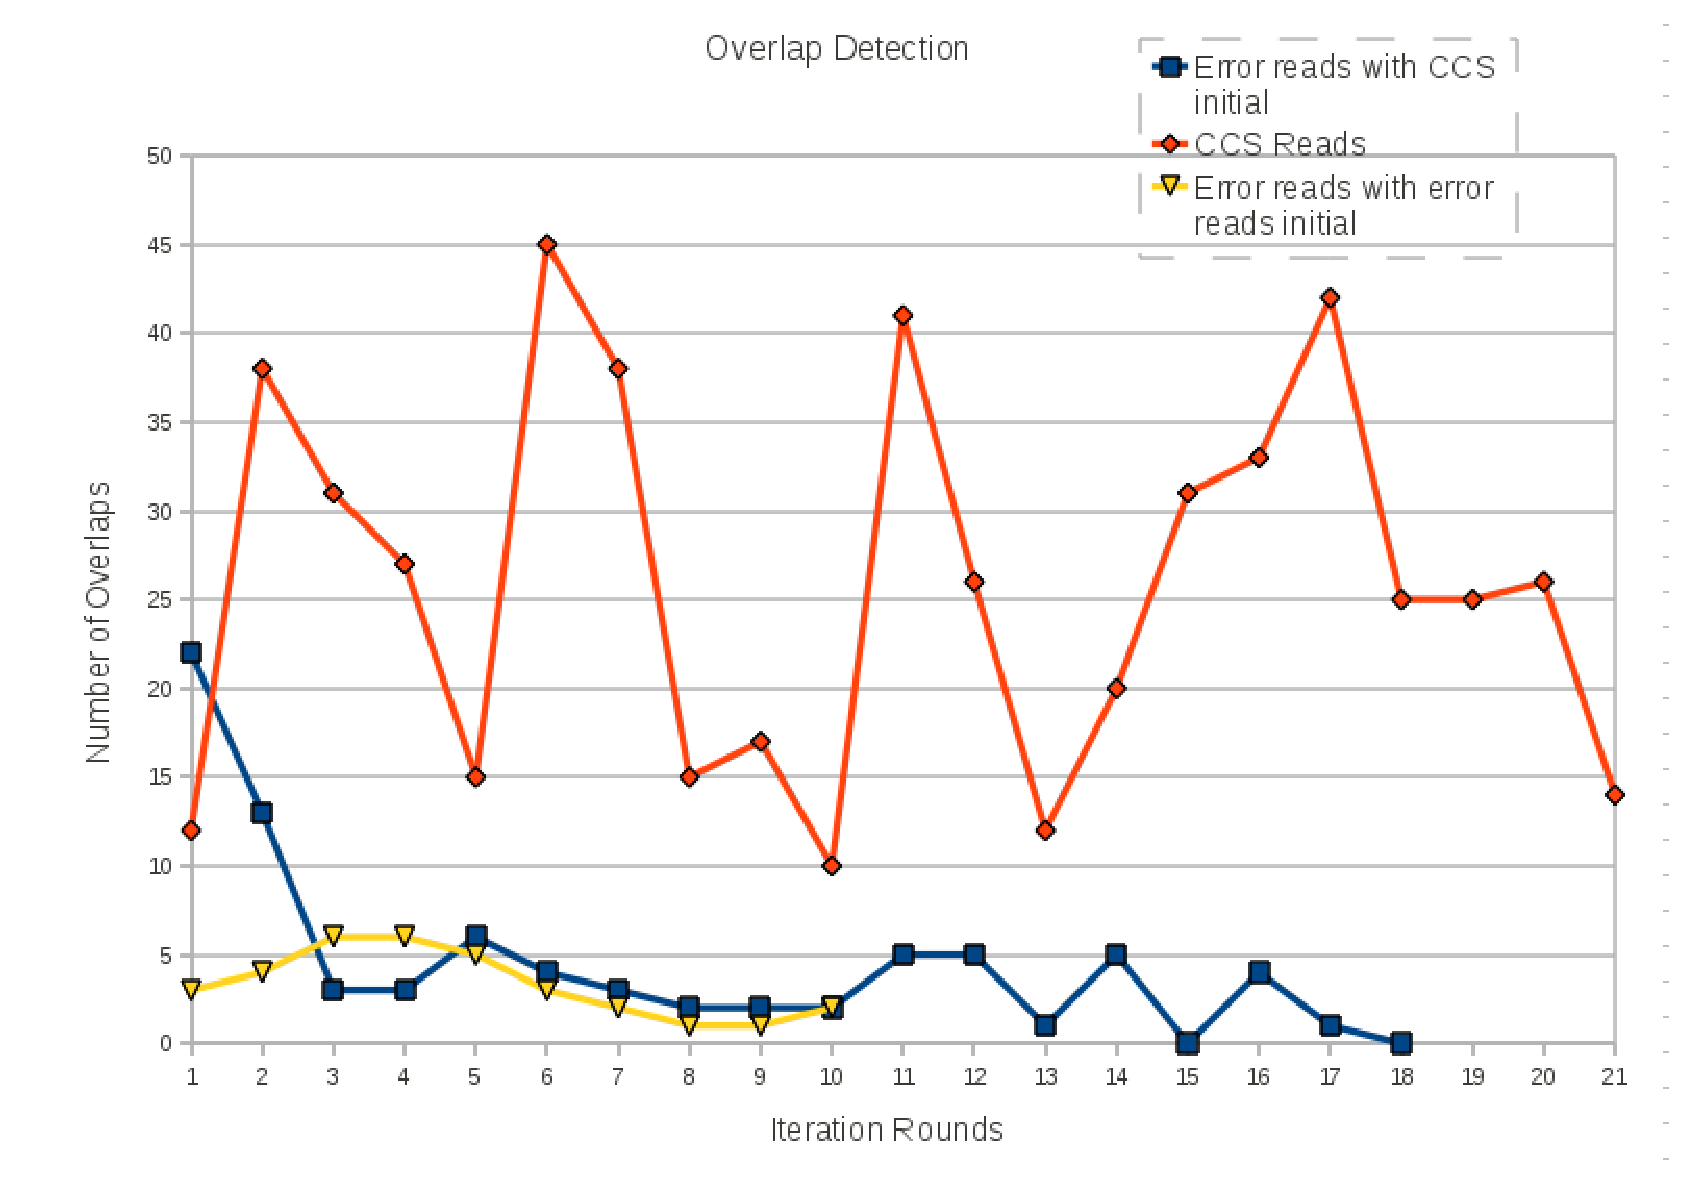
\includegraphics[width=12.5cm, keepaspectratio=true]{overlap.eps}
    \caption{\label{fig:overlap}Overlap detection}
\end{figure}

\subsection{Experiment on CCS reads}

When applied to CCS reads, the reference grows quickly and steadily, as shown in
Figure \ref{fig:ccs}.  After 36 rounds the reference becomes 251159-base-long.
The average distance is only 0.0142 per matched base.

\begin{figure}[t]
    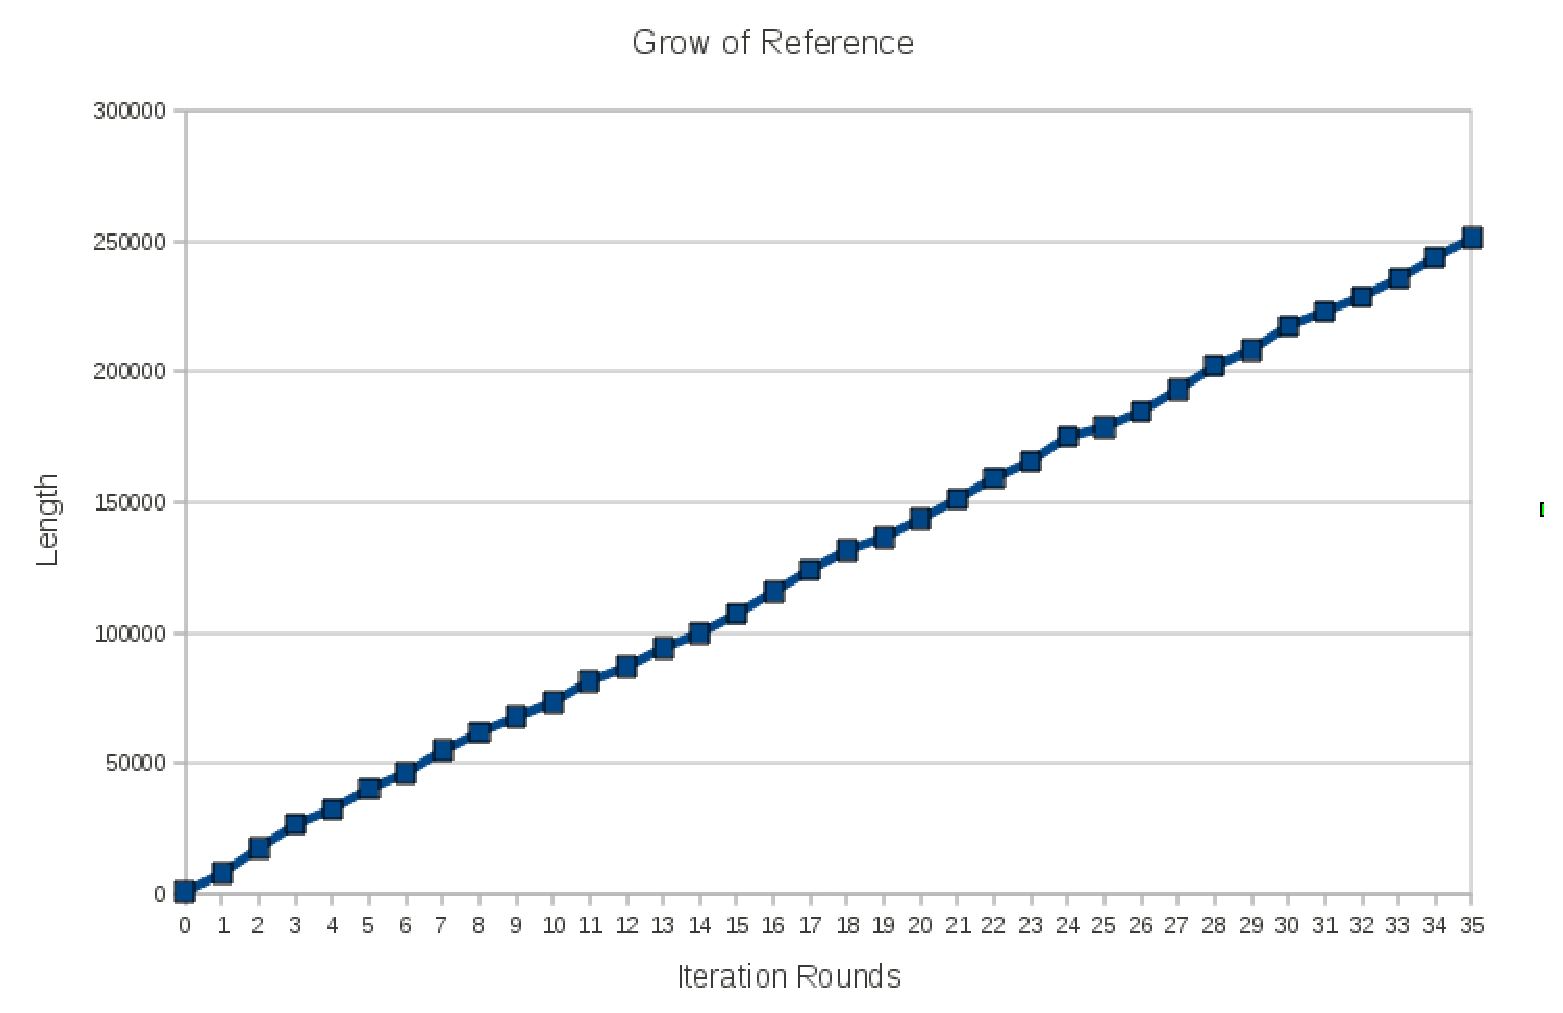
\includegraphics[width=12.5cm, keepaspectratio=true]{ccs.eps}
    \caption{\label{fig:ccs}Reference growth on CCS reads}
\end{figure}

\subsection{Experiment on error reads}

When applied to error reads, its biggest difference between the experiment on
CCS reads is the number of overlaps is much smaller. When the iteration goes
deeper, the risk of detecting 0 overlap increase. In that case, the iteration
has to stop. By far, the longest sequence we have achieved is of length 120914.
The growth of the reference is presented in Figure \ref{fig:real}. 

To evaluate the effect of error correction, we would like to compare our result
with the contig results provided by PacBio. However, even with a distance of
10\%, the complexity of this comparison is $0.1 \times 600000^2 = 3.6 \times
10^{10}$, which is apparently prohibitive on our machine. Instead, we estimate
the error rate of the assembly result by aligning the CCS reads against it.
Because CCS reads are of very high accuracy, the distance between CCS reads and
the assembly can be a good estimate. For the 120914-long-contig, the error rate
is 0.1219. The length of the contig is significantly larger than reads and the
error rate is also significantly decreased compared to the 0.15 average. It is
also worthy notice that this result is obtained with an initial error reads,
     namely, no CCS corrected reads but only the long reads with high error are
     used. This result is also available at the website of source code. 

\begin{figure}[t]
    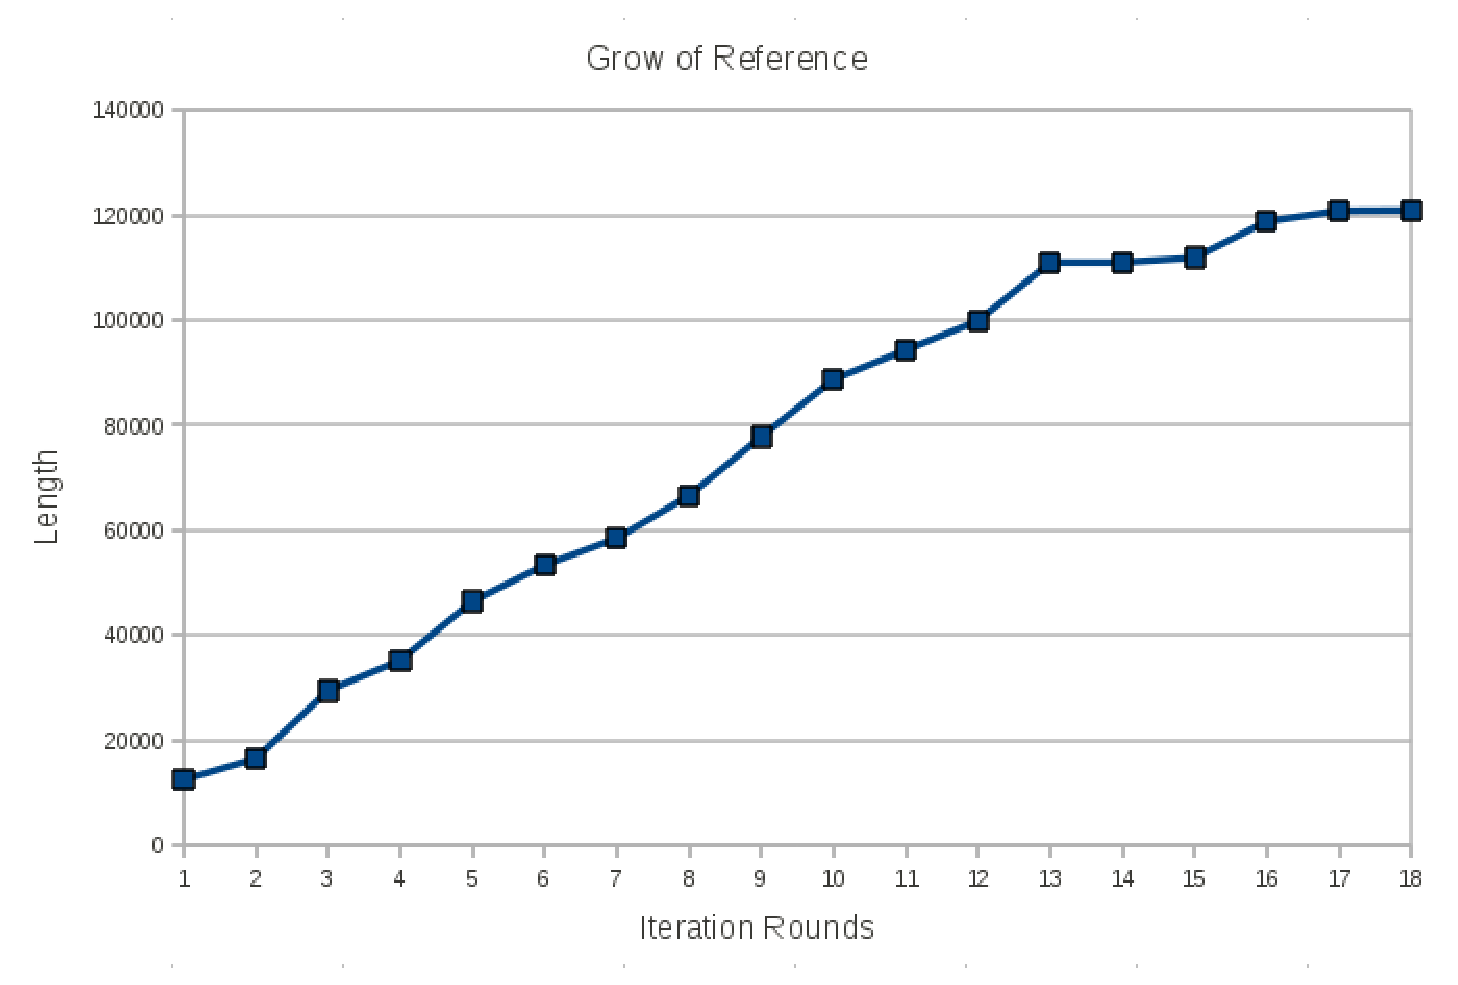
\includegraphics[width=12.5cm, keepaspectratio=true]{real.eps}
    \caption{\label{fig:real}Reference growth on long reads with high error rate}
\end{figure}

\section{Conclusion}

In our project, we implemented an assebly program that try to build the genome
of E. coli from PacBio's long reads with high error rate. The critical point of
the program is to find overlap. A seed-and-expand algorithm is used to get a
concensus from aligned segments, so that errors can be corrected. Our program is
successful in detecting overlaps and expand the reference. We achieved a
120914-long-contig with 0.1219 error rate. However, to assemble the whole genome
using only the high error rate long reads, more overlaps should be found.

\section{References}

{[}Altschul 1990{]} S. F. Altschul, W. Gish, W. Miller, E. Myers, D. J.
Lipman, Basic local alignment search tool, J. Mol. Biol., 215 (1990),
403--410. \\

{[}Ma 2002{]} B. Ma, J. Tromp, M. Li, Pattern Hunter--faster and more
sensitive homology search. Bioinformatics, 18 (2002), 440--445. \\

{[}Keich 2004{]} U. Keich, B. Ma, M. Li, and J. Tromp, On spaced seeds
for similarity search, Discrete Applied Mathematics 138 (3) (2004),
253--263. \\

{[}Choi 2003{]} K. Choi, F. Zeng, and L. Zhang, Good spaced seeds for
homology search. Bioinformatics 20 (2003), 1053--1056. \\

{[}Ukkonen 1985{]} E. Ukkonen, Algorithms For Approximate String
Matching, Information and Control, 64 (1985), 100--118. \\

{[}Roover 2005{]} C. De Roover, C. De Vleeschouwer, F. Lefebvre, B.
Macq, Robust video hashing based on radial projections of key frames,
IEEE Transactions on Signal Processing, 53 (10), 2005, 4020--4037. \\

{[}Pevzner 2001{]} P. A. Pevzner, H. Tang, and M. S. Waterman. 2001, A
New Approach to Fragment Assembly in DNA Sequencing, Proceedings of the
Fifth Annual International Conference on Computational Biology (RECOMB
'01), New York, NY, 256--267.

\end{document}
